\documentclass{article}

\usepackage{graphicx}
\usepackage{float}

\graphicspath{{pictures/}}

\author{Joshua Reed}
\title{Cooper Mountain Nature Park}


\begin{document}
\maketitle{}
\section{Structural}
\subsubsection{Abiotic}\label{ssub:abiotic}
There are many structures of this habitat that allow it to function. One such structure
is the larder shown in figure~\ref{larder}. This particular larder was built by humans,
but natural larders are found throughout the area.
\begin{figure}[H]
\centering{}
\caption{A Man Made Larder}
\includegraphics[scale=0.07]{larder.jpg}
\label{larder}
\end{figure}
\newpage

In this instance of abiotic structure a pile of rocks is a possible home to 
reptilian organisms. The sign in figure~\ref{rocks} reads please do not disturb. 
Sensitive reptile research underway.
\begin{figure}[H]
\centering{}
\caption{Reptile Rocks}
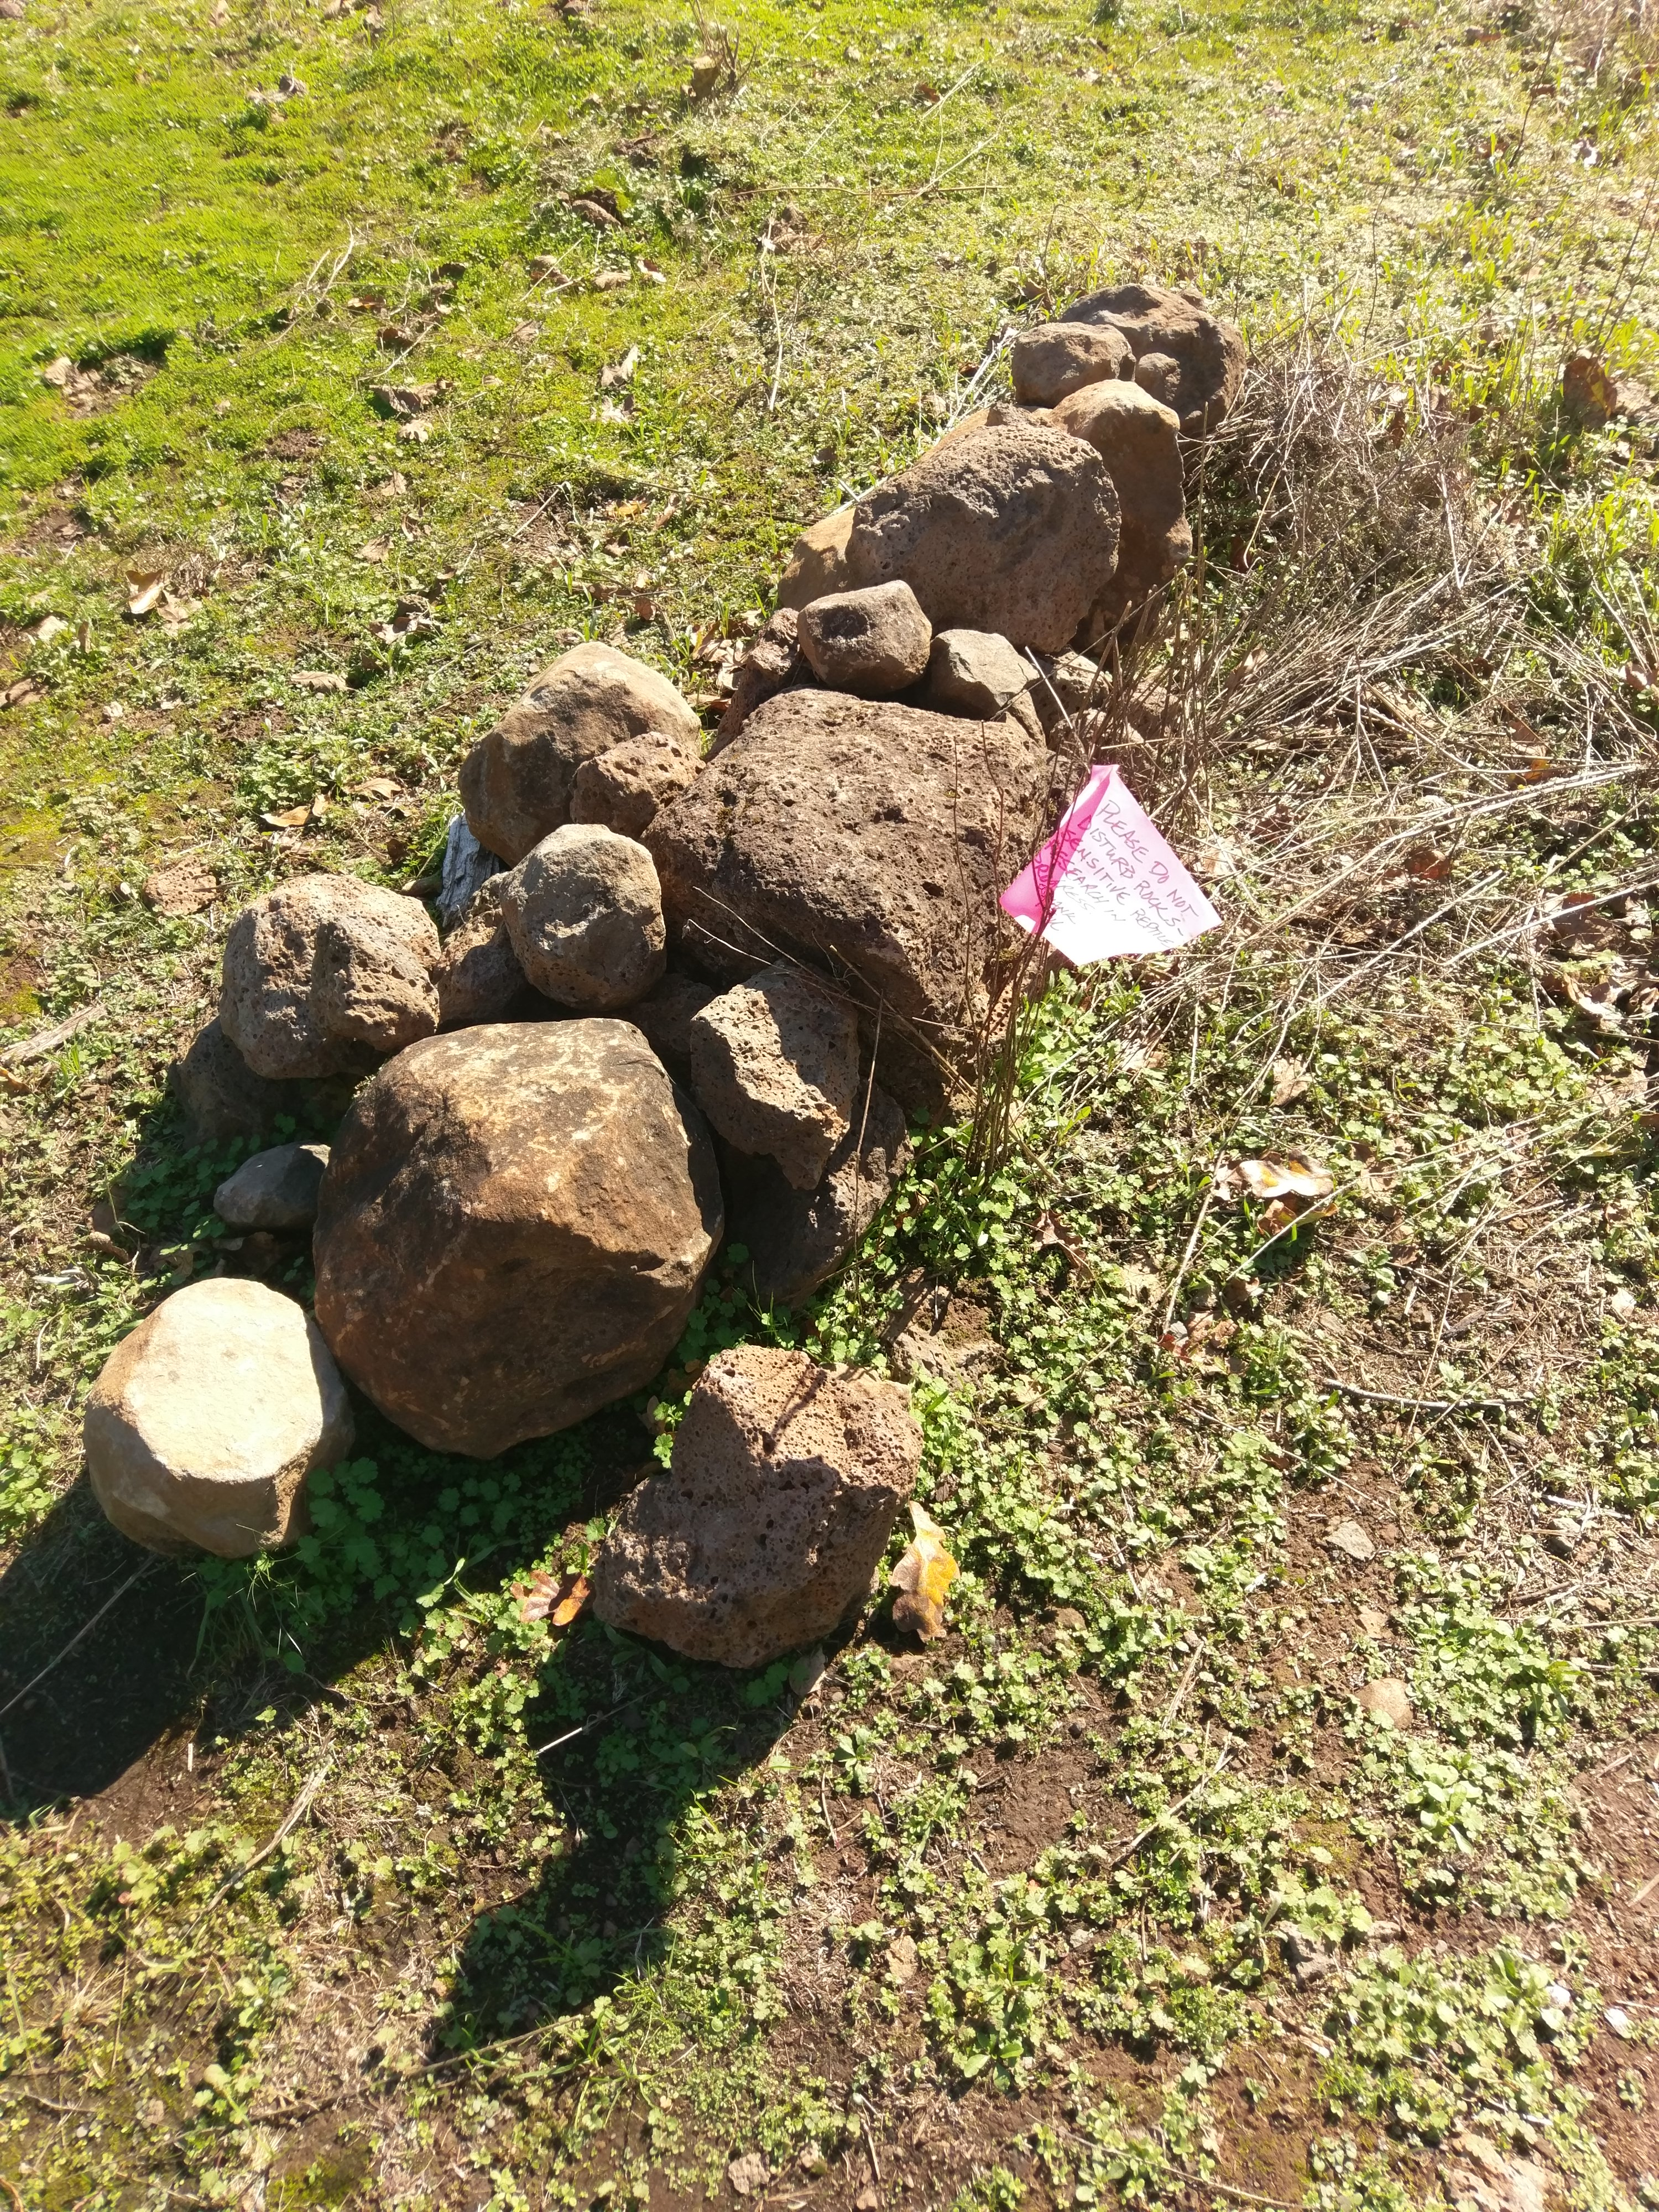
\includegraphics[scale=0.07]{reptile_research.jpg}
\label{rocks}
\end{figure}


\subsubsection{Soils}
A proper soil mixture allows plants to take place after primary and secondary succession.
This ecosystem underwent primary succession long long ago, but as I  write about
below, secondary succession is common to this ecosystem due to fire. 

Today, the plants thrive in a healthy topsoil, and their root systems help to prevent 
errosion. 

\newpage

\subsection{Biotic}\label{ssub:biotic}
This nature park was home to many organisms. Figure~\ref{tracks} shows a key to some of 
the tracks that can be spotted within the park grounds. From Deer to Bears, this park
is home to a variety of creatures.

\begin{figure}[H]
\centering{}
\caption{Tracks On Sign}
\includegraphics[scale=0.07]{animal_tracks.jpg}
\label{tracks}
\end{figure}
\newpage
Unfortunately the time of day I went there wasn't much wildlife present. As such, 
I wasn't able to get a good photo of any animals. I did see several birds though.
Also, there were several very informative signs with pictures of animals.
\begin{figure}[H]
\centering{}
\caption{Bear on Sign}
\includegraphics[scale=0.06]{bears_eat_berries_sign.jpg}
\label{bear}
\end{figure}

\begin{figure}[H]
\centering{}
\caption{Squirrel on Sign}
\includegraphics[scale=0.06]{grey_squirrel_sign.jpg}
\label{squirrel}
\end{figure}
\newpage


Further still, there were many plants that provide both habitat and food as primary 
producers within the park. Some of them can be seen in figures~\ref{barkless} to~\ref{berry}
\begin{figure}[H]
\centering{}
\caption{Evergreen Trees}
\includegraphics[scale=0.07]{some_evergreens.jpg}
\label{barkless}
\end{figure}

\begin{figure}[H]
\centering{}
\caption{Deciduos Tree}
\includegraphics[scale=0.07]{fall_leaves.jpg}
\label{}
\end{figure}

\begin{figure}[H]
\centering{}
\caption{Fern}
\includegraphics[scale=0.06]{fern.jpg}
\label{}
\end{figure}

\begin{figure}[H]
\centering{}
\caption{Flowering Grass}
\includegraphics[scale=0.06]{grass_inflourecense_closeup.jpg}
\label{}
\end{figure}

\begin{figure}[H]
\centering{}
\caption{Grass}
\includegraphics[scale=0.06]{thin_grass_inflorecense_closeup.jpg}
\label{}
\end{figure}

\begin{figure}[H]
\centering{}
\caption{Bush with Red Berries}
\includegraphics[scale=0.06]{red_berry_bush.jpg}
\label{berry}
\end{figure}
\newpage

Still further detritivores are a big part of the parks ecosystem.

\begin{figure}[H]
\centering{}
\caption{Fungi}
\includegraphics[scale=0.05]{mushrooms1.jpg}
\label{fungi}
\end{figure}

\begin{figure}[H]
\centering{}
\caption{Fungi on Wood}
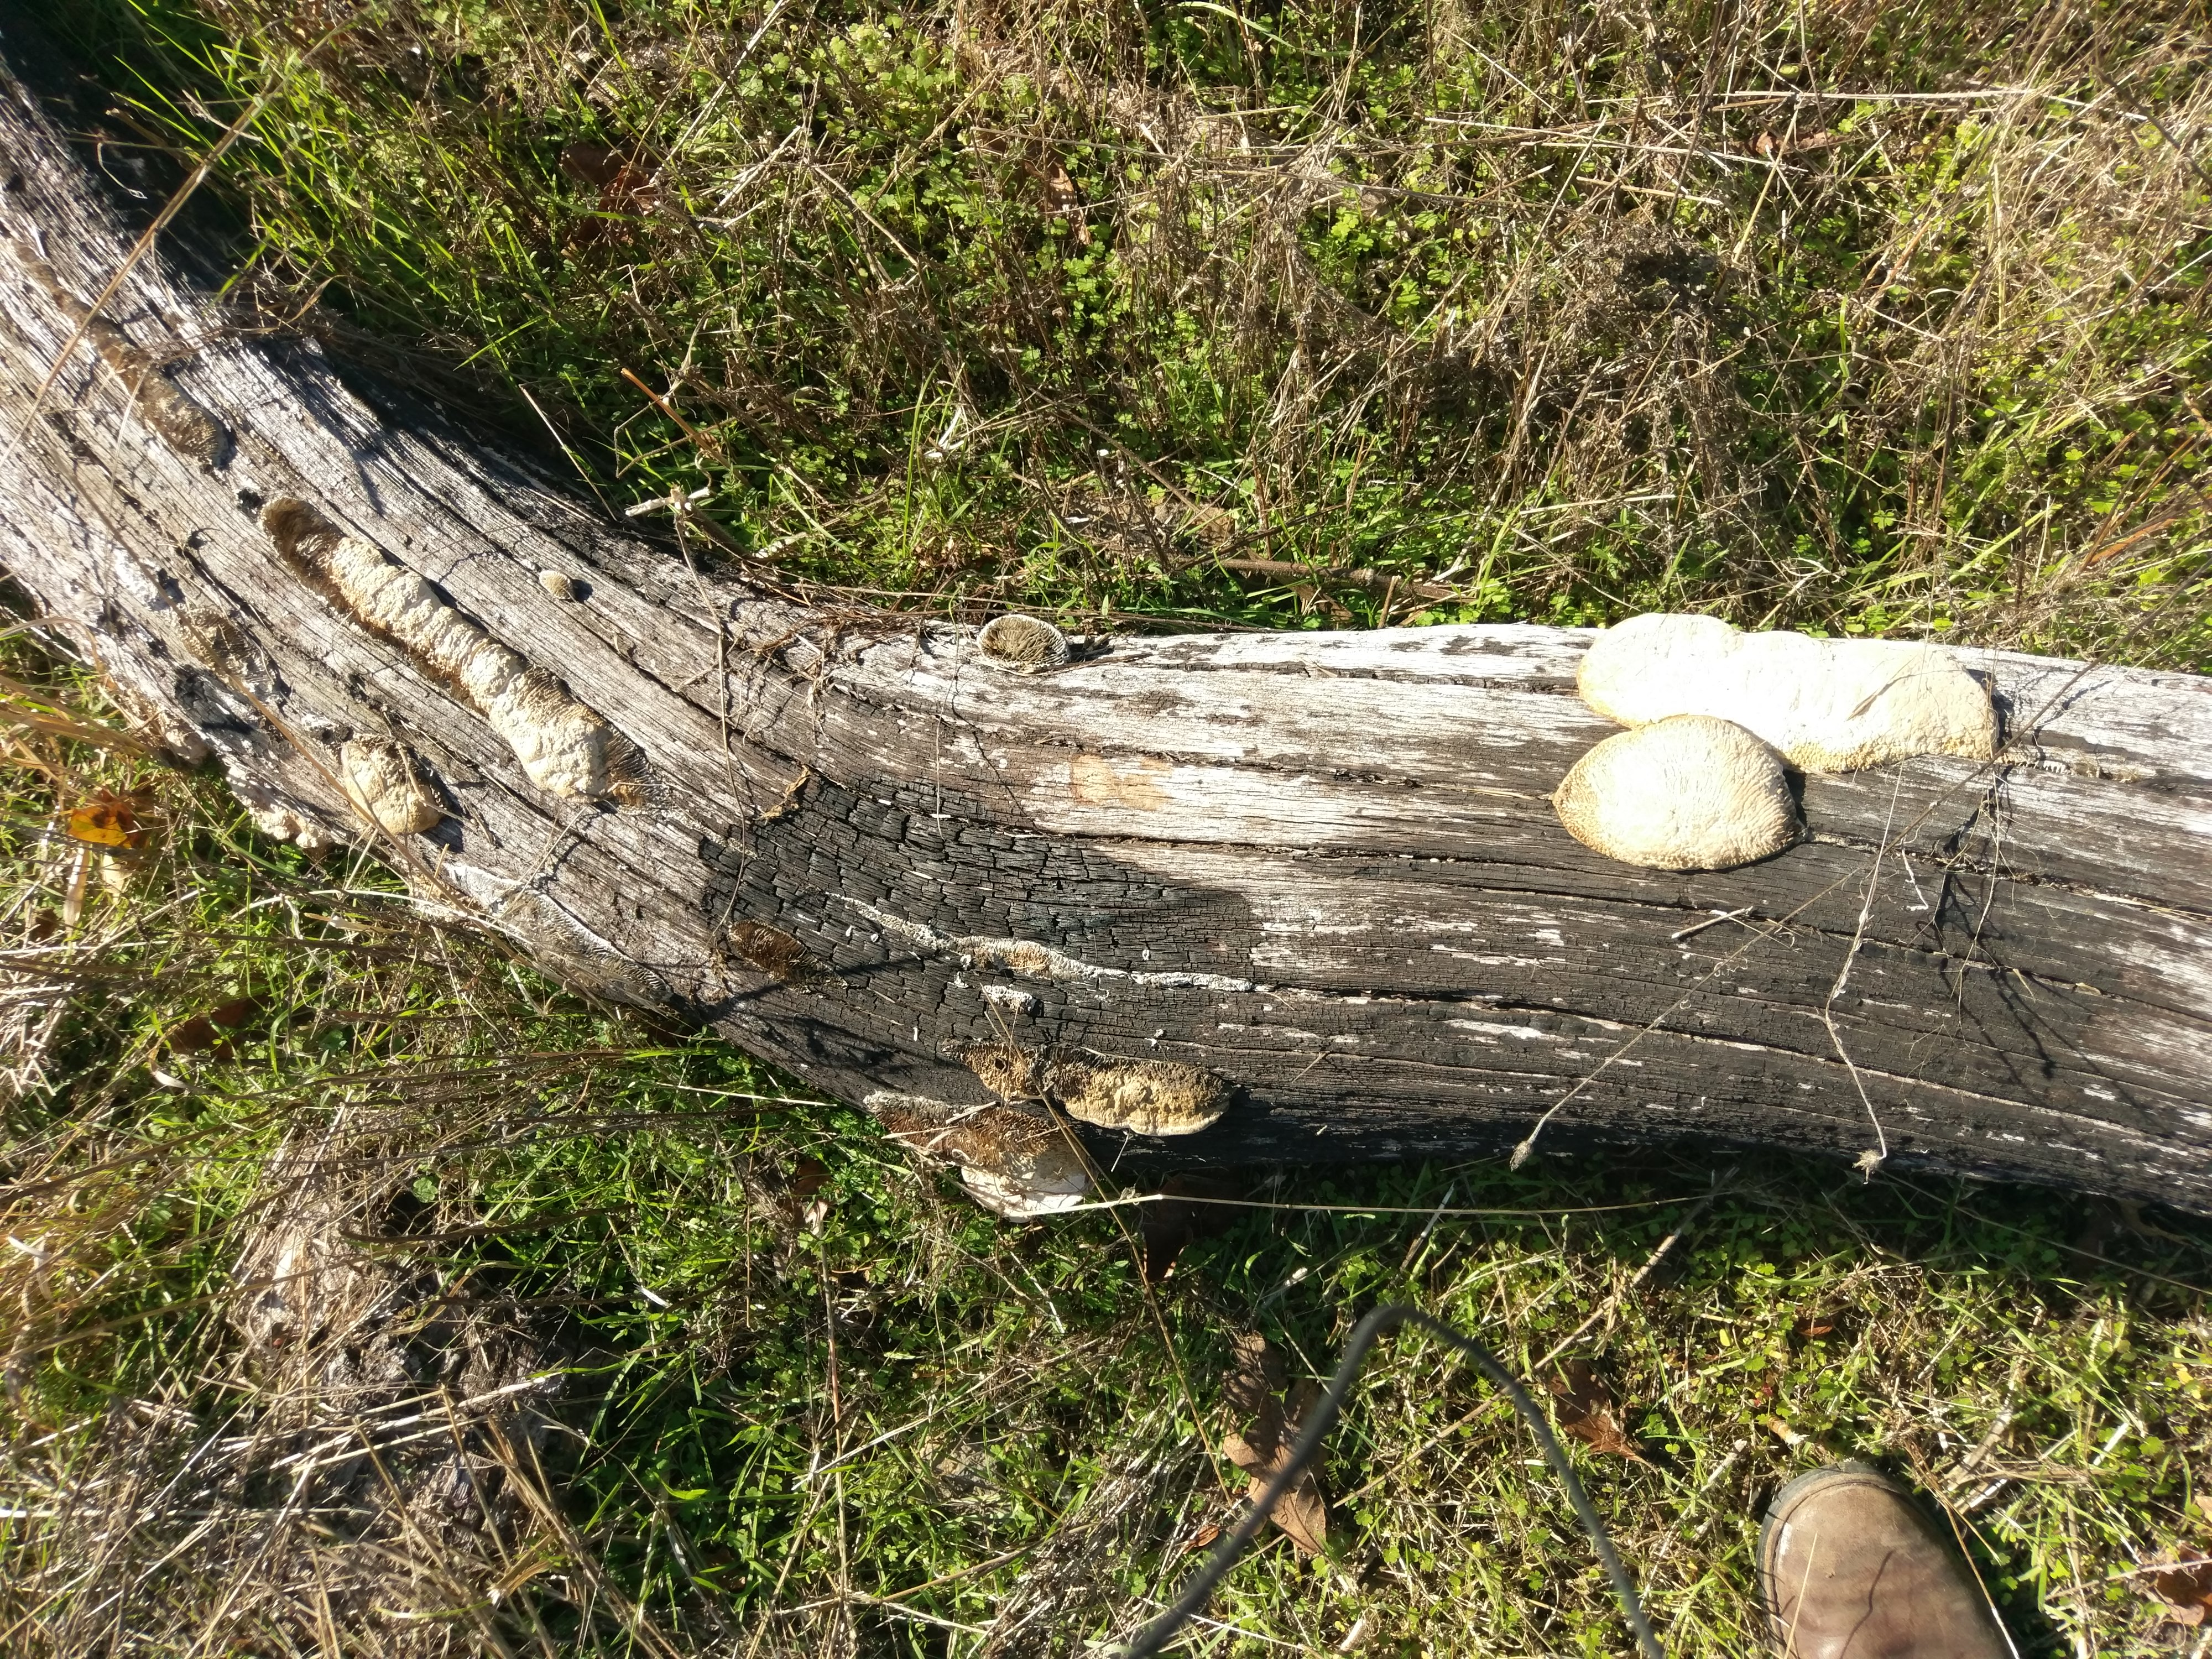
\includegraphics[scale=0.05]{burntwood_with_fungi.jpg}
\label{fungi}
\end{figure}
\newpage

\section{Controls}
\subsection{Weather}
\subsubsection{Temperature}\label{ssub:temperature}
Temperature clearly affects the animals and plants within the park. For example, 
deciduous trees lose their leaves in the winter as an adaptation to the cold. A warmer
spring will cause plants to grow more quickly. 

\subsubsection{Precipitation}\label{ssub:temperature_label_ssub_temperature}
It was a bright and calm day when I visited, but all of the grenery wouldn't exist without
precipitation. For that mater without the water cycle including transpiration, precipitation, and evaporation, none of this system would function.

\subsubsection{Wind}\label{ssub:temperature_label_ssub_temperature}
A lot of plants require wind to help them dispurse their seeds. Beyond this, wind can
help a fire to grow. 

\subsection{Area}
The park is fairly large at 231 acres, but as shown in figure~\ref{area}, 231 acres
isn't exactly a large area when it comes to supporting the natural habitat of some 
species. This could also be considered an abiotic structural influence.
\begin{figure}[H]
\centering{}
\caption{Area Required}
\includegraphics[scale=0.05]{size_to_support_sign.jpg}
\label{area}
\end{figure}
\newpage


\subsection{Disturbances}
\subsubsection{Fire}\label{ssub:fire}
Fires are a natural cyclical disturbance of this habitat. In this area a fire could be expected at least every five years. 
Today fires are controlled in many ways, and still used to control invasive species and 
help natural species to flourish. As shown in the sign below, fire is essential 
in maintaining this ecosystem.
\begin{figure}[H]
\centering{}
\caption{Fire Sign}
\includegraphics[scale=0.05]{fire_renews_the_prarie.jpg}
\label{fire}
\end{figure}

The sign in figure~\ref{fire} states that the area was last burned in 2008.

\begin{figure}[H]
\centering{}
\caption{Burnt Wood}
\includegraphics[scale=0.05]{burntwood.jpg}
\label{}
\end{figure}

\begin{figure}[H]
\centering{}
\caption{Burnt Wood With Fungi}
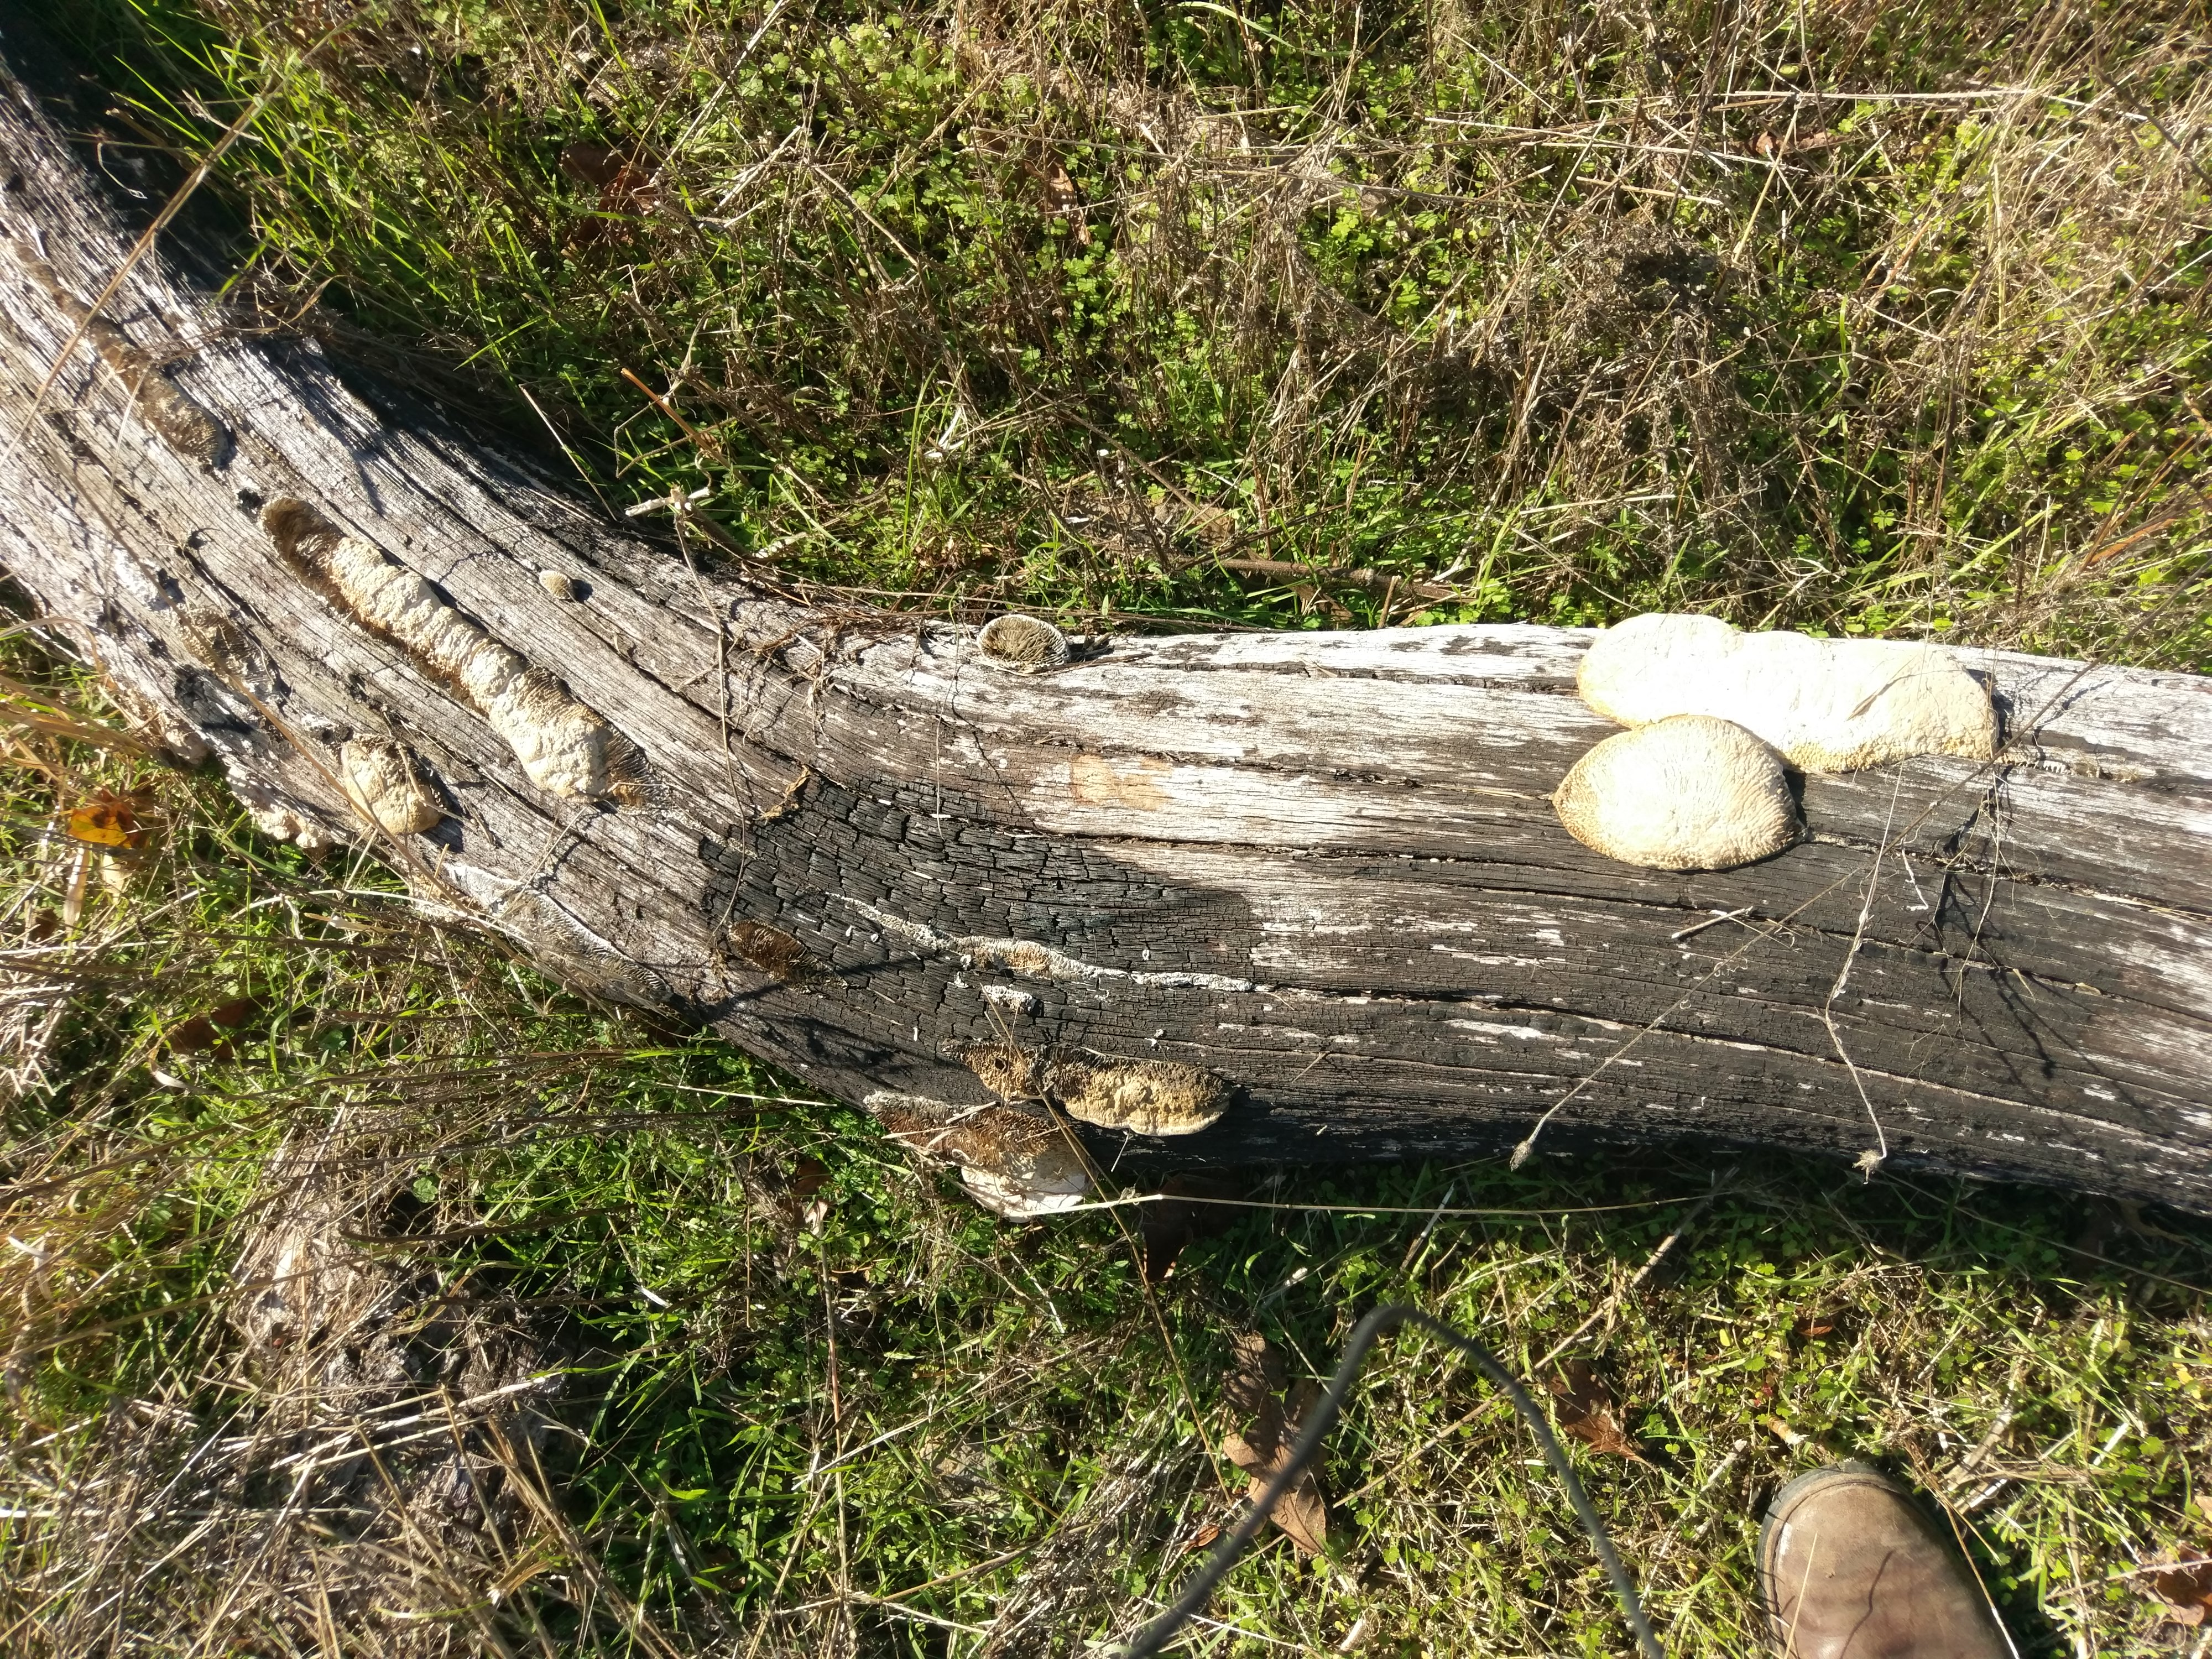
\includegraphics[scale=0.05]{burntwood_with_fungi.jpg}
\label{}
\end{figure}
\newpage


\subsubsection{Invasive Species}\label{ssub:invasive_species}
Shown in figure~\ref{dandy} is a dandelion found along the trail. At this stage in the parks
development it seems fairly unlikely that dandelions would become a truly invasive
species, but during secondary succession I'm sure the park is quite sensitive to 
invasive species like these.

\begin{figure}[H]
\centering{}
\caption{Dandelions}
\includegraphics[scale=0.05]{dandelions.jpg}
\label{dandy}
\end{figure}

Invasive species is clearly a concern for the parks management as can be seen in figure~\ref{shoes}.
\begin{figure}[H]
\centering{}
\caption{Clean your Shoes!}
\includegraphics[scale=0.07]{stowaway_seeds_sign.jpg}
\label{shoes}
\end{figure}
\newpage

And while not an invasive species, dogs aren't allowed in the park as much of the
wildlife views them as predators. It is believed that dogs would make wildlife sparce.
\begin{figure}[H]
\centering{}
\caption{No Dogs}
\includegraphics[scale=0.08]{no_dogs_sign.jpg}
\label{dogs}
\end{figure}
\newpage

\section{Conclusion}
I had no idea there was a park this cool less than 3 miles from my house! I'm really 
grateful to have learned of and about it because of this project. Beyond all of the 
awesome nature, it is simply a beautiful place to be.

\begin{figure}[H]
\centering{}
\caption{Beatiful Oak Grove}
\includegraphics[scale=0.065]{oak_woodlands1.jpg}
\label{}
\includegraphics[scale=0.065]{oak_woodlands2.jpg}
\end{figure}

\end{document}
